% % % % % % % % % % % % % % % % % %
%                                 %
%    PROJECT REPORT - GROUP 16    %
%    Nisheeth Lahoti 110050027    %
%    Shivam H Prasad 110050041    %
%    Sheetal Godara  110050014    %
%                                 %
% % % % % % % % % % % % % % % % % %

\documentclass[a4paper,11pt]{article}
\usepackage[top=0.6in, bottom=1in, left=0.5in, right=0.5in]{geometry}
\usepackage{graphicx}

\begin{document}
	\title{\textbf{Rube Goldberg Project Analysis:\\ A CS296 Group 16 Report.}}
	
	\author {
		Nisheeth Lahoti\\ Roll no. 110050027\\ \emph{lahoti@cse.iitb.ac.in}
		\and Shivam H Prasad\\ Roll no. 110050041\\ \emph{shivamh@cse.iitb.ac.in}
		\and Sheetal Godara\\ Roll no. 110050014\\ \emph{sheetal@cse.iitb.ac.in}
	}
	
	\date{January 25, 2013}
	\maketitle
	
	\section{Introduction}
		The pupose of this report is to analyse various aspects of the Rube
		Goldberg Machine simulation. We describe the initial design that was
		proposed, the changes made to the design, analysis of the time taken for
		different parts of the program and an overview of optimizations involved.
	
	\section{Initial and Final Designs}
		The purpose of our Rube Goldberg machine is to lift a box that has fallen
		in a pit. (Which was originally planned to be  a car that fell into a
		pond).\\
		
		This was the design first proposed by our group -
			\begin{center}
				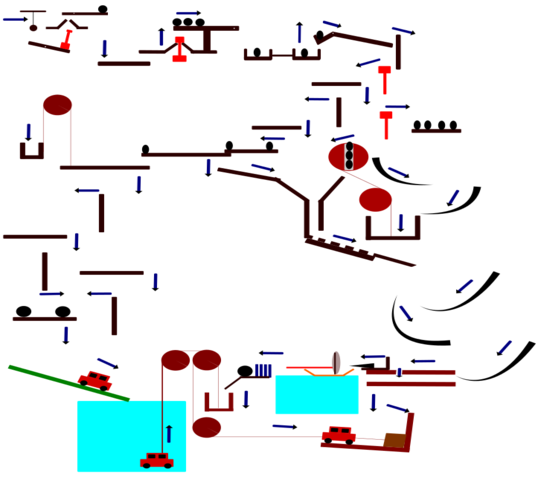
\includegraphics[scale=0.7]{./doc/images/initial_design.png}
			\end{center}
		
		We made the following changes to the original design (for primarily two
		reasons - either the unavailability of a feature in Box2D, or to avoid
		the simulation becoming unnecessarily repetetive and cumbersome) -
		\begin{itemize}
			\item \textbf{Fewer curves and planks in the ball's path:} Originally,
			there were a large number of curves and planks (to bring the ball down
			from a height) which didn't actually affect the complexity of the
			design itself. So we removed the un-necessary parts wherever we felt
			that a single curve or plank would suffice - leaving the design as
			complicated as it was before, while making it less cumbersome.
			
			\item \textbf{Removal of two or three features:} One of the features
			included in the initial design - a pulley which contained three balls
			in its centre - can apparently not be made in Box2D. Besides, we
			made one grave mistake in the original design - we unnecessarily
			included an apparatus for pushing the car in the water. We decided it
			made more sense to omit this part in the final.
			
			\item \textbf{Changed the starting apparatus of the simulation:} The
			original starting appratus involved, among other things, a plank that
			had to be balanced with a weight on one side. This, as far as we could
			find out, cannot be done reliably in Box2D. So we had to change the
			entire starting appratus - though we tried to retain as much
			superficial similarity as possible.
			
			\item \textbf{Change in appearance of a few objects:} There was no way
			to render a car or a boat in Box2D. So what looks like a car in the
			initial design becomes a box in the final, and what looks like a boat
			becomes a simple structure made up of three rods.
		\end{itemize}
		
		In the end, this was the design actually prepared -
			\begin{center}
				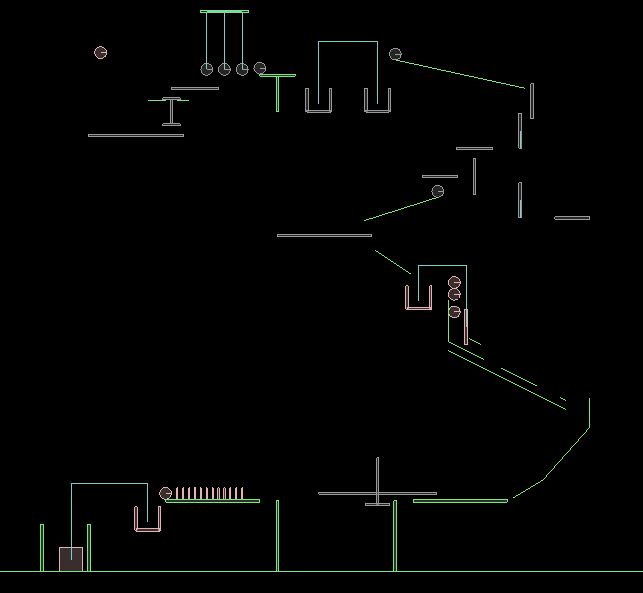
\includegraphics[scale=0.7]{./doc/images/final_design.png}
			\end{center}
	
	\section{Time Analysis}
		Several processes involved in the simulation have been timed over various
		number of iterations, the program being run many number of times for each
		iteration, to obtain a large sample. Also, the program has been run under
		different loads on the CPU, and in different versions.\\
		The following conclusions can be drawn from the five plots:
		
		\subsection{Total Loop Time}
			\begin{center}
				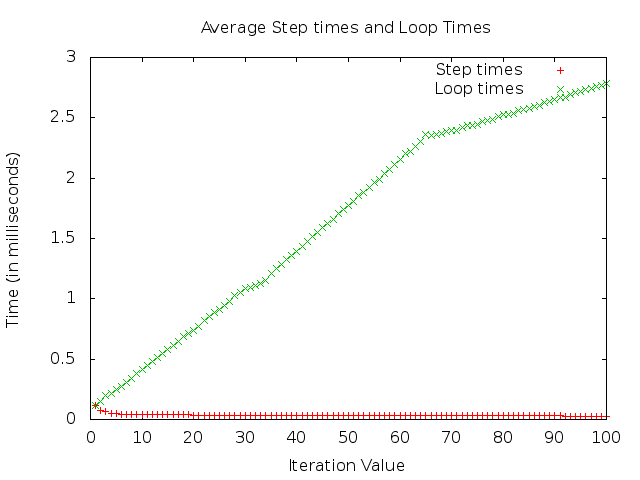
\includegraphics[scale=0.5]{./doc/images/g16_plot01.png}
			\end{center}
			
			As can be seen, the total loop times are roughly in one straight line
			from the $1^{st}$ to the $65^{th}$ iteration, and in another straight
			line from $65^{th}$ iteration onwards. To understand this, we checked
			out the executable, which explains this behaviour simply -
			\begin{itemize}
				\item Till the $30^{th}$ step, no object had settled. So
				in every loop the program considered the possibility of collision of
				every single object, and hence had to update positions and velocities
				of each one.
				\item In the $30^{th}$ step, all the planks and some containers
				"settled down". However, all these were the objects which were not
				colliding before anyway. So, the overall velocity update time did
				not change (since these were not contributing to it), but the
				position update time reduced (since they were moving slightly).
				\item However, as seen from the next graph, velocity update time
				for all iterations is almost thrice as large as position update
				time. So, despite the position update time being halved, total time
				for each step did not change much at all.
				\item In the $65^{th}$ step, the dominoes settled down. These,
				unlike the planks, were indeed colliding (with the floor). So, the
				total velocity update time dropped drastically, reducing the total
				step time considerably.
				\item No further 'activation/deactivation' of any object occurred
				after the $65^{th}$ step. So, the time required for each individual
				step again became a constant, leading to a straight line behaviour
				of the total time required upto the $n^{th}$ step, for $n>65$.
			\end{itemize}
		
		\subsection{Average times over steps}
			\begin{center}
				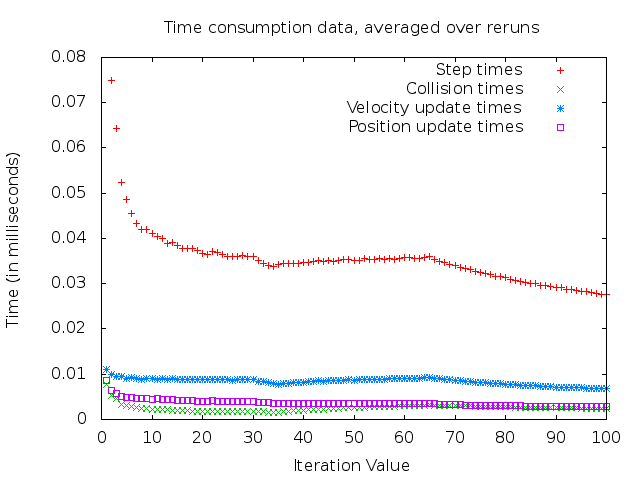
\includegraphics[scale=0.5]{./doc/images/g16_plot02.png}
			\end{center}
			
			The variation in these average times can be understood directly using
			the previous graph. Time required for the first step is naturally
			higher than the other steps, since the program has to call various
			constructors and load positions and velocities as opposed to
			incrementally updating them. Then for the next few steps, due to the
			nearly constant time required for each step, the total loop time takes
			the form $ax+b$, with a small $b$ (Since $b$ is the extra time
			required for the first step). So the average times are of the form
			$a+\frac{b}{x}$. The small value of $b$ implies that the graph appears
			to fall for some time and then becomes constant. After 30 steps, due
			to the reduction in slope of total time, the graph takes the form
			$cx+d$, with a relatively large $d$. So, the graph appears roughly
			hyperbolic.
		
		\subsection{Variations over reruns}
			\begin{center}
				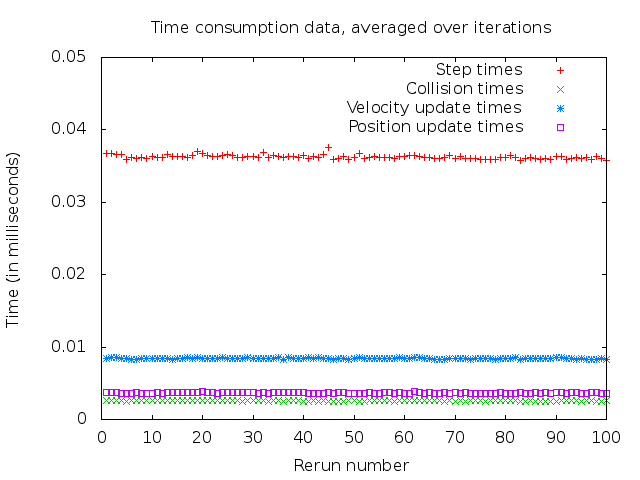
\includegraphics[scale=0.5]{./doc/images/g16_plot03.png}
			\end{center}
			
			Hardly anything surprising here. However, if we run the simulation
			when the CPU is under considerable load, one interesting difference
			arises. The average time becomes about twice as much. Also, the graph
			often goes below the average level, but seldom above.
			The most reasonable  guess we could make is that the modal level
			occurs when the CPU (which is dual core) is able to devote one core to
			the program. Reductions in time taken represent those relatively rare
			instances when both the cores are free.
		
		\subsection{Error bars for step times}
			\begin{center}
				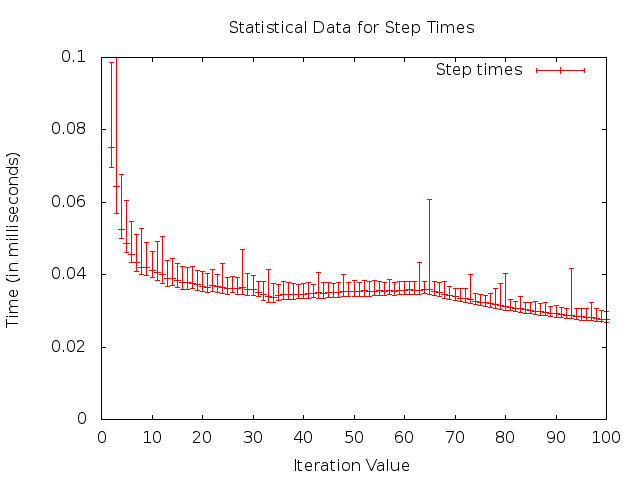
\includegraphics[scale=0.5]{./doc/images/g16_plot04.png}
			\end{center}
			
			The most noticeable aspect of this plot is the reduction in the sizes
			of the error bars. Well, there's obviously the reason that the values
			themselves decrease, so even at the same relative error, the error
			bars would have got smaller. But that's not \emph{exactly} the case -
			here, even the relative error is decreasing. This too, however, is
			expected. As we can see from the previous graph, the CPU is mostly at
			one particular speed. For natural numbers $0<a<b<100$, the average
			speed for any $a$ iterations would naturally show more relative
			variation than the average speed for $b$ iterations. So, we would have
			a higher chance of observing a significantly different time for the
			first $a$ iterations than for the first $b$.
		
		\subsection{Frequency of step times}
			\begin{center}
				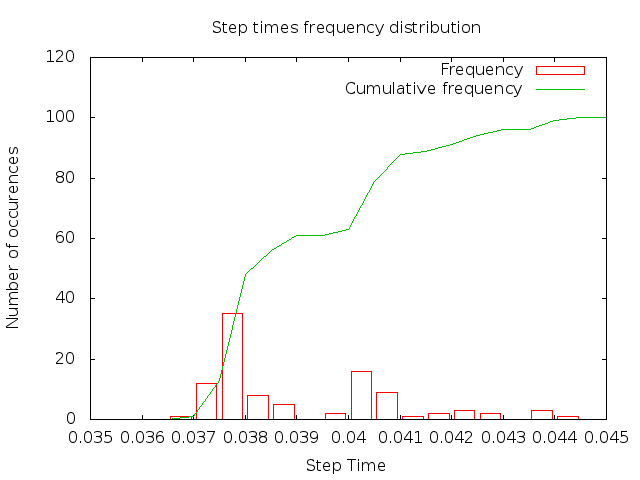
\includegraphics[scale=0.5]{./doc/images/g16_plot05.png}
			\end{center}
			
			Most of the values here are concentrated in a small range (0.036 to
			0.042). This would be because the data for this graph is the time
			for the same iteration (number 14) over different reruns. As seen
			in graph $\#3$, that does not vary considerably.
	
	\section{Optimization}
		We have not done any optimization in the code itself, since the inbuilt
		optimizations provided by compilers have done quite a good job of
		reducing running time. Box2D has been installed in the Release mode, and
		the source code has been compiled with the O3 flag. Besides elementary
		optimizations, this flag copies the code for most functions into the code
		of the caller, which results in expansion of the code but reduces the
		time taken (as function calls are avoided). Since there are no recursive
		functions anywhere in our project, this means the function calls have
		been removed altogether in the executable, leading to an extremely fast
		and low-memory program.
\end{document}

